\title{Self-consistent Green's function approaches}
\author{Carlo~Barbieri and Arianna Carbone}
\institute{
Carlo Barbieri  \at 1 Department of Physics, University of Surrey, Guildford GU2 7XH, UK \email{C.Barbieri@surrey.ac.uk},
\and Arianna Carbone   \at 2 Institut f�r Kernphysik, Technische Universit�t Darmstadt, 64289 Darmstadt, Germany, and 
\\ ExtreMe Matter Institute EMMI, GSI Helmholtzzentrum f�r Schwerionenforschung GmbH, 64291 Darmstadt, Germany, \email{arianna@theorie.ikp.physik.tu-darmstadt.de},
}
\maketitle
\abstract{
We present the fundamental techniques and working equations of Green's function methods for calculating of ground state properties and of the spectral strength distribution in finite and infinite fermionic systems.  We follow an approach based on the self-consistent calculation of many-body propagators and derive the working equations for the one-body Green's function, using both the Algebraic Diagrammatic Construction (ADC) technique and the self-consistent formalism  at finite temperature. Green's function methods closely relate to the polynomial scaling approaches discussed in Chapters ??  and  ??.  However, it leads to a global view of the many-fermion structure.
 The third order ADC approach [ADC(3)] is the method of choice for handling finite nuclei and can also be applied to  infinite systems by discretising the single particle Hilbert space in momentum coordinates. As a related numerical project, we describe the construction of a complete numerical code for infinite neutron and nuclear matter.
We then focus on how to approach calculations at finite temperature which do not require a discretisation of the Hilbert space. The self-consistency feature is essential to guarantee thermodynamic consistency and details of the inclusion of three-nucleon interactions are also discussed.}


\section{Introduction}

Ab-intio methods that present polynomial scaling with the number of particles have proven highly useful in reaching
finite systems of rather large sizes (as for medium mass nuclei) and even infinite matter. Most approaches of this type that are discussed in Previous chapters discuss techniques that aims at the direct evaluation of the ground state energy of the system, where several other quantities of interests can be addressed in a second stage through the equation of motion and particle removal or attachment techniques.
%
In this chapter, we will follow a different route and focus on gaining a global overall view of the spectral structure of a system offermions. Our approach will be that of calculating directly the self-energy (a.k.a. mass operator) that describes the 
complete response of a particle embedded in the true ground state of the system. This not only provides an optical potential for elastic scattering but it also provide spectral information for the attachment and removal of a particle.   Once one body Green's function as been obtained the total energy of the system is calculated---as the final step---by means of appropriate sum rules.

Two main approaches have become standard as standard choices for calculations in Nuclear many-body theory.
\hbox{~~~~~~~~~~~~} 
The Algebraic Diagrammatic Construction (ADC) methods has proven to be optimal for discrete bases, as it is normally necessary to exploit for finite systems. However this can also be applied to fermion gasses in a box with periodic boundary conditions, which even simplifies application thanks to translational invariance. We will focus on the case on infinite nucleonic matter and provide an example of a working numerical code.
\hbox{~~~~~~~~~~~~}
The other method consists in solving directly the nucleon-nucleon ladder scattering matrix for dressed particles in the medium, which can be done effectively in a finite temperature formalism. Thus, this allows for studying thermodynamic properties of the infinite and liquid matter. For this studies to be reliable it is mandatory to ensure the satisfaction fundamental conservation principle and to satisfy conservation laws and maintain thermodynamic consistency in the infinite size limite. We show here how to achieve this by preforming fully self-consistent calculations of the Green's function (hence the name SCGF).
\hbox{~~~~~~~~~~~~}\\
Very recent advances in computational applications concern the extension of SCGF theory to the Gorkov-Nambu formalism for the breaking on particle number symmetry. This allows to  treat pairing systematically in degenerate (i.e. not closed shell) systems. Hence, has opened the possibility of  studying large set of semi-magic nuclei that were previously beyond the reach of ab-initio theory. We will not discuss the Gorkov-SCGF approach here and focus on the fundamental features of the standard approaches instead. The interested reader is referred to  recent literature on the topic.

We introduce the concept of many-particle Green's function in Section~\ref{sec:scgf_defs} and discuss the relation between the one-body spectral function and experimental data. This will also allow us to cover the main sum rules needed to extract the total binding energy of the system and any one-body observable.
 The ADC(n) method is explained in Sec.~\ref{sec:scgf_adc}, where all working equations up to third order are derived.  We demonstrate how to apply this in a calculation of infinite matter in  Sec.~\ref{sec:scgf_comp} by using a simplified two-nucleon interaction. This section will give insight on how to construct the corresponding C++ code included with this book.
The finite temperature formalism is then introduced in Sec.~\ref{sec:scgf_finiteT} together with working equation used as standard in the nuclear physics literature.
%
Further details of the implementation of chiral 3NF in the finite temperature formalism are given in  Appendix 1.


\section{Many-body Green's function theory}
\label{sec:scgf_defs}


In this chapter will focus on the one-body green's function, which is also the simplest 
example of many-body Green's function (or propagator). This is define below here:
\begin{equation}
 g_{\alpha, \beta}(\omega) = 
\end{equation}
In spite of this being the simplest type of propagator, it does contain a wealth of information
regarding single particle behaviour inside the many-body system, on one-body observables,
on the total binding energy, and even elastic nucleon-nucleus scattering.

We will discuss the $g_{\alpha, \beta}(\omega)$ for a general case of 3NFs and introduce the 
Dyson equation, which is the central equation for the whole theory.





\subsection{Spectral function and relation to  experimental observations}

Here we summarize the spectral function and its relation to one- body observables,  the
density matrix $\rho({\bf r})$ and  modification to the Koltun sum rule in presence of 3NFs.

\subsection{Perturbation expansion of the Green 's function}

In order to understand the following sections and to devise appropriate approximations to the self-energy,
in is necessary to understand the basics elements of perturbation theory.  These will be also fundamental to 
derive all-order summation schemes leading to non perturbative solutions and to discuss the concept
of self-consistency.

We summarize here the material needed to understand the following sections, while the full set of Feynman rules
is reviewed in  Appendix 2


\section{The Algebraic Diagrammatic Construction method}
\label{sec:scgf_adc}

The general Lehman representation of the self-energy is given by~\eqref{}, where $\Sigma^{(\infty)}$  is given by the mean-field diagram of Fig.~\ref{}. Similarly to the case of a propagator, Eqs.~\eqref{} and~\eqref{}, the  pole structure of the energy-dependent part is dictated by the principle of causality with the correct boundary  coded by the  $\pm i\eta$ terms at the denominators.  This implies a dispersion relation that  can links the real and imaginary parts of the self-energy.  Correspondingly, the direct coupling single particle orbits to  ISCs (of 2p1h and 2h1p character of more complex) imposes  the separable structure of the residues. In this section we consider that case of a  finite system, for which it is useful to use a discretised single particle basis as a model space. Thus, the above constraints impose the following  analytical form the the self energy operator:
\begin{equation}
\Sigma^{(\star)}(\omega) = \Sigma^{(\infty)} +M\frac1{\omega - E -C + i \eta}M +N\frac1{\omega - E -D + i \eta}N
\label{eq:ADC_SE_form}
\end{equation}
where the indices $r$ and $n$ label set of configurations beyond SP structure. Specifically, $r$ is for particle addition and will label 2p1h, 3p2h, 4p3h, ... states---although our discussion below will only be limited to 2p1h. Likewise, $n$ is for particle removal and we will used it to label 2h1p states (or higher configurations, in general).


The expansion of the self-energy at second order in PT trivially satisfies Eq.~\eqref{eq:ADC_SE_form}. By simple comparison with the results 
of Eq.~\eqref{eq:Sig_2nd} shows us that the $r\equiv{n_1,n_2,k_3}$ us to Now we can identify the matrix expressions for the matrix elements of the residues and poles as follows:
\begin{eqnarray}
 M_{\alpha,r} &=&
 \nonumber \\
 E_{r,r'} &=& diag \left\{ \,\varepsilon^+_{n_1} + \varepsilon^+_{n_2} - \varepsilon^-_{k_3}  \, \right\}
 \nonumber \\
 C_{r,r'} &=& 0
 \label{eq:ADC2_MC}
   \\
 N_{\alpha,s} &=&
 \nonumber \\
 E_{s,s'} &=& diag \left\{ \, \varepsilon^-_{k_1} + \varepsilon^-_{k_2} - \varepsilon^+_{n_3} \, \right\} 
 \nonumber \\
 D_{s,s'} &=& 0
  \label{eq:ADC2_ND}
\end{eqnarray}
where the factor $1/2$ in Eq. disappears since we restrict the sums to triplets of indices where  $n_1<n_2$ and $k_1<k_2$.
As we discuss below, Eqs~.\eqref{eq:ADC2_MC} and \eqref{eq:ADC2_ND}, define the algebraic diagrammatic method
at second order [ADC(2)].


Unfortunately, $\Sigma$ loses its analytical form of Eq.~\eqref{eq:ADC_SE_form} as soon as one moves to higher orders in PT. 
To demonstrated this, let us calculate the contribution of the 3rd order 'ladder' diagram of Fig.xx. by exploiting Feynman rules
and Eq.~\ref{} we obtain
\begin{eqnarray}
  \Sigma^{??}(\omega) &=& \int \frac{d\omega_1}{2\pi} \int \frac{d\omega_1}{2\pi} \int \frac{d\omega_1}{2\pi} v_{,} g_{}(\omega_1 - \omega_2)  g_{}(\omega_2) v_{,} g_{}(\omega_1 - \omega_3)  g_{}(\omega_3) v_{,} g_{}(\omega) 
\nonumber \\
  &=& \int \frac{d\omega_1}{2\pi}  v_{,}  g_{}(\omega_1)  v_{,}   g^{IIf}_{}(\omega_1) v_{,} g_{}(\omega_1 - \omega) 
\nonumber \\
  &=& \int \frac{d\omega_1}{2\pi}  v_{,}  
   \left\{ \frac{\pazocal{X}\pazocal{X}  \pazocal{X}\pazocal{X}}{\omega_1 - e^+_{n_1} - e^+_{n_2} + i\eta} 
        - \frac{\pazocal{Y}\pazocal{Y}  \pazocal{Y}\pazocal{Y}}{\omega_1 - e^-_{k_1} - e^-_{k_2} - i\eta}  \right\}
        v_{,}  \left\{ \frac{\pazocal{X}\pazocal{X}  \pazocal{X}\pazocal{X}}{\omega_1 - e^+_{n_4} - e^+_{n_5} + i\eta} 
        - \frac{\pazocal{Y}\pazocal{Y}  \pazocal{Y}\pazocal{Y}}{\omega_1 - e^-_{k_4} - e^-_{k_5} - i\eta}  \right\}
     \nonumber \\
 && \quad   v_{,}  
   \left\{ \frac{\pazocal{X}  \pazocal{X}}{\omega_1 - \omega  - e^+_{n_3} + i\eta} 
        + \frac{\pazocal{Y}  \pazocal{Y}}{\omega_1 - \omega  - e^-_{k_3} - i\eta}  \right\} \; .
        \label{eq:LaddEg1}
 \end{eqnarray}
 By applying the Cauchy theorem, only six term out of the eight combination of poles survive. To simplify the discusssion 
 we will focus only on the three integrals that contribute to the forward propagation of the self-energy (send term on the r.h.s.
 of \eqref{eq:ADC_SE_form}). This is done by retaining only the poles $(\omega_1 - \omega  - e^-_{k_3} - i\eta)^{-1}$ in the
 last propagator of Eq.~\eqref{eq:LaddEg1}, which lie above the real axis with respect to the integrand $\omega_1$. Thus,
 we have:
 \begin{eqnarray}
  \Sigma^{??}(\omega) &=& \int \frac{d\omega_1}{2\pi}  v_{,}  
   \left\{ \frac{\pazocal{X}\pazocal{X}  \pazocal{X}\pazocal{X}}{\omega_1 - e^+_{n_1} - e^+_{n_2} + i\eta}      \right\}
     v_{,}  
      \quad   \left\{  \frac{\pazocal{Y}\pazocal{Y}  \pazocal{Y}\pazocal{Y}}{\omega_1 - e^-_{k_4} - e^-_{k_5} - i\eta}  \right\}
 v_{,}  
   \left\{  \frac{\pazocal{Y}  \pazocal{Y}}{\omega_1 - \omega  - e^-_{k_3} - i\eta}  \right\} \; .
     \nonumber \\
&&+
\int \frac{d\omega_1}{2\pi}  v_{,}  
   \left\{ \frac{\pazocal{Y}\pazocal{Y}  \pazocal{Y}\pazocal{Y}}{\omega_1 - e^-_{k_1} - e^-_{k_2} - i\eta}  \right\}
 v_{,}  
 \quad   \left\{ \frac{\pazocal{X}\pazocal{X}  \pazocal{X}\pazocal{X}}{\omega_1 - e^+_{n_4} - e^+_{n_5} + i\eta}   \right\}
 v_{,}  
   \left\{ \frac{\pazocal{Y}  \pazocal{Y}}{\omega_1 - \omega  - e^-_{k_3} - i\eta}  \right\} \; .
     \nonumber \\
&&+
\int \frac{d\omega_1}{2\pi}  v_{,}  
   \left\{ \frac{\pazocal{X}\pazocal{X}  \pazocal{X}\pazocal{X}}{\omega_1 - e^+_{n_1} - e^+_{n_2} + i\eta}   \right\}
     v_{,}  
      \quad   \left\{ \frac{\pazocal{X}\pazocal{X}  \pazocal{X}\pazocal{X}}{\omega_1 - e^+_{n_4} - e^+_{n_5} + i\eta}    \right\}
 v_{,}  
   \left\{\frac{\pazocal{Y}  \pazocal{Y}}{\omega_1 - \omega  - e^-_{k_3} - i\eta}  \right\} \; .
        \label{eq:LaddEg2}
        \nonumber \\
  &=&  \quad
 \nonumber \\
   &&+~
    \nonumber \\
   &&+~
    \nonumber \\
  &\equiv& \quad M^{(2,ld)}\frac1{\omega - E + i \eta}M^{(1)}
  \nonumber \\
   &&+~  M^{(1)}\frac1{\omega - E + i \eta}M^{(2,ld)}
  \nonumber \\
   && +~  M^{(1)}\frac1{\omega - E + i \eta}C^{(ld)}\frac1{\omega - E + i \eta}M^{(1)}  \; ,
 \end{eqnarray}
where $M^{(1)}$ and $E$ come from Eq.~\eqref{eq:ADC2_MC}. The 2p1h ladder interaction $C^{(ld)}$ is at first order in $V$, while the coupling matrix $ M^{(2,ld)}$ is at second order. These can be read from the previous lines of Eq.~\eqref{} and turn out to be:
\begin{eqnarray}
M^{(2,ld)}_{\alpha,r} &=&
  \nonumber \\
  C^{(ld)}_{r,r'} &=& \pazocal{X}\pazocal{X}  v_{,}  \pazocal{X}\pazocal{X}  \, \delta_{k_3, k_3'} \; .
\end{eqnarray}

Eq.~\eqref{eq:LaddEg2} is clearly breaks the known Lehman representation for the Self-energy and would even lead to inconsistent 
results unless its contribution is very small compared to the second order contribution of Eq.~\ref (that is, approximation would
break unless $V$ is perturbatively small).
Therefore, we need to identify proper corrections that allows to retain these 3rd order contributions but at the same time let
us recover the analytical form of~\eqref{eq:ADC_SE_form}.  For the first two terms on the right hand side of Eq.~\eqref{eq:LaddEg2}, this
issue can be easily solved by remembering that the corresponding diagram from $\Sigma^{(2)}(\omega)$ [see Eq.~\eqref{}] is to be included.
If then one adds an extra term that is quadratic in  $M^{(2,ld)}$, this lead to:
\begin{eqnarray}
  \Sigma^{(2)}(\omega)  ~+~ \Sigma^{(3, ld)}(\omega) ~+~ M^{(2,ld)}\frac 1 {\omega  - E + i\eta} M^{(2,ld)}
 % \nonumber \\
 \longrightarrow  \left[ M^{(1)} +  M^{(2,ld)}\right] \frac1{\omega  - E + i\eta}\left[ M^{(1)} + M^{(2,ld)}\right]  \; ,
\end{eqnarray}
which resolves the issue of obtaining the residues in separable form. Note that this new correction is one specific Goldstone diagram that
appears in the {\em fourth order} expansion of the self-energy. On the other hand, adding all of the fourth order diagrams would lead to 
new term that break themselves the Lehman representation and that in turn would require selected Goldstone terms at even higher orders to be
corrected.  In other words, we have achieved to recover the structure of Eq.~\eqref{eq:ADC_SE_form}  but at the price of giving up a systematic 
perturbative expansion that is complete at each order in $V$. Given that the Lehman representation is dictated by physical properties, this is 
a more satisfactory rearrangement of the perturbation series.

The last term in Eq.~\eqref{eq:LaddEg2} is more tricky to correct since it contains second order poles as $(\omega  - E - i\eta)^{-2}$, which cannot be 
cancelled by single contributions at higher order. Instead, we are forced to perform a non-perturbative resummation of Goldstone diagrams to all orders that results in a geometric series. This is done by considering the relation
\begin{equation}
 \frac1{A-B}  ~=~  \frac1 A ~+~ \frac1 A  \, B \,  \frac1{A-B}  ~=~  \frac1 A  ~+~  \frac1 A  \, B \,  \frac1 A  ~+~  \frac1 A  \, B \,   \frac1 A   \, B \,   \frac1 A
             ~+~ \frac1 A  \, B \,  \frac1 A  \, B \,  \frac1 A  \, B \,  \frac1 A  ~+ \ldots
  \label{eq:1overAB}
\end{equation}
for two operators $A$ and $B$. If we chose  $A\equiv{\omega  - E + i\eta}$ and $B\equiv C$,  the first and second term on the right hand 
side can then be  identified with the contribution from $\Sigma^{(2)}(\omega)$ and the  last term of Eq.~\eqref{eq:LaddEg2}. 
Also in this case, all perturbative terms up to third order have been kept unchanged  but ....

In the end the forward ladder terms in the self energy become
If then one adds an extra term that is quadratic in  $M^{(2,ld)}$, this lead to:
\begin{eqnarray}
  \Sigma^{(2)}(\omega)  ~+~ \Sigma^{(3, ld)}(\omega) ~+~ \begin{array}{c} \hbox{terms beyond} \\ \hbox{ 3$^{rd}$ order } \end{array} 
  \nonumber 
 \longrightarrow  \left[ M^{(1)} +  M^{(2,ld)}\right] \frac1{\omega  - E - C^{(ld)} + i\eta}\left[ M^{(1)} + M^{(2,ld)}\right]  \; ,
\end{eqnarray}


{\bf Exercise 11.1}.  Complete  the calculation of Eq.~\eqref{} and derive the remaining corrections to the 2h1p interaction $D^{(ld)}$  and the 1h-2h1p coupling term  $N^{(2,ld)}$.


\subsection{The algebraic diagrammatic construction method}

 The  procedure discussed above to devise proper approximations of the self-energy is at the heart of the
 algebraic diagrammatic construction  (ADC) method, originally introduced b J. Schirmer and collaborators~\cite{}.
 This approach  generates  a hierarchy of approximations of increasing accuracy such that,
 at a given order $n$, the ADC($n$) equations will maintain the analytic form of Eq.~\eqref{eq:ADC_SE_form} and
 also contain the full Feynman expansion for $\Sigma^\star(\omega)$ up to order $n$.
 %
 
In order to do this, we expand the Lahman representation in powers of the perturbatin interactions $V$. The interaction matrices 
$C$ and $D$ appearing in the denominators can only be of first order in $V$. However, the coupling matrices can contain terms
of any order:
\begin{eqnarray}
  M &=& M^{(1)} +  M^{(2)} +  M^{(3)} +  \ldots
   \nonumber  \\
  N &=&  N^{(1)} +  N^{(2)} +  N^{(3)} + \ldots
 \label{eq:MNexp}
\end{eqnarray}
By using  Eqs.~\eqref{eq:1overAB}  and~\eqref{eq:MNexp} we see that the energy dependent
part of the self-energy appears only starting from the second order. The corresponding expansion
of Eq.~\ref{eq:ADC_SE_form} is
\begin{eqnarray}
  \Sigma^{\star}(\omega) &=&  \Sigma^{(\infty)}
  \nonumber \\
   &+& M^{(1)}\frac1{\omega - E -C + i \eta}M^{(1)} +N^{(1)}\frac1{\omega - E -D + i \eta}N^{(1)}
    \nonumber \\
  &+&~ M^{(2)}\frac1{\omega - E + i \eta}M^{(1)}  +   M^{(1)}\frac1{\omega - E + i \eta}M^{(2)}
%  \nonumber \\
%   &&
 +  M^{(1)}\frac1{\omega - E + i \eta} C \frac1{\omega - E + i \eta}M^{(1)}  
    \nonumber \\
  &+&~ N^{(2)}\frac1{\omega - E + i \eta}N^{(1)}  +   N^{(1)}\frac1{\omega - E + i \eta}N^{(2)}
%  \nonumber \\
%   &&
 +  N^{(1)}\frac1{\omega - E + i \eta} D \frac1{\omega - E + i \eta}N^{(1)}  \
 \nonumber \\
 &+& \ldots
 \label{eq:ADC_SE_form_exp}
\end{eqnarray}
The ADC procedure is then to simply calculate the analitic expression of all possible diagrams up
to order $n$. By comparing these to the expansion~\eqref{eq:ADC_SE_form_exp} one then reads
the minimum expressions for the coupling and interaction matrices, M, N, C and D that are needed to
include all the $n$-order diagrams. Correspondingly, the energy-independent self-energy $\Sigma^{(\infty)}$
needs to be expanded at least up to order $n$ as well.
 Note that the dynamic part of the self-energy appears, which propagates ISCs, appears only starting from the
 second order. This is so because any diagram needs one perturbing interaction $V$ to generate an ISC
 and a second one to annihilate it back to a single particle state. In general, if the Hamiltonian contains
 up to $m$-body forces and $i$ an integer numbers then the ADC($2i$) and ADC($2i+1$) will require
 ISCs up to  [($m$-1)*$i$+1]-particle--($m$-1)*$i$-hole and [($m$-1)*$i$+1]-hole--($m$-1)*$i$-particle.
 Thus with two-nucleon forces ADC(2) and ADC(3) include  2p1h and 2h1p states,  ADC(4) and ADC(5) include 
 3p2h and 2h3p states, and so on. However, the full ADC(2/3) sets with three-nucleon forces already
 requires 3p2h and 3h2p configurations.

At frist order, ADC(1) require to only calculate diagram(s) that contribute to $\Sigma^{(\infty)}=\tilde{U}$,
see Fig.xx, and thus the scheme reduces to HF theory.
At second order and with a two-body interaction, there is only one diagram contributing to $\tilde\Sigma(\omega)$
which is already in the proper Lehman form. Hence, Eqs.~\ref{eq:Sig_2nd},~\ref{eq:ADC2_MC} and~\ref{eq:ADC2_ND}
fully define the ADC(2) approximation. In this case, $\Sigma^{(\infty)}$ also require a second order non-skeleton term.

Higher order cases are more complicated. For a two-body Hamiltonian, the only non-skeleton diagrams at third order
are the ladder and ring diagrams shown in Fig.xx.  As long as one works with fully self-consistent (dressed)
propagators or with an HF reference state these are sufficient. In this cases additional  non-skeleton terms vanish and
do not need to be included (see Exercise 11.3).
Assuming that this is the case, one obtains the following working expressions the for the ADC(3) approximation:
\begin{eqnarray}
 M_{\alpha,r} &=&
 \nonumber \\
 E_{r,r'} &=& diag \left\{ \,\varepsilon^+_{n_1} + \varepsilon^+_{n_2} - \varepsilon^-_{k_3}  \, \right\}
 \nonumber \\
 C_{r,r'} &=& 0
 \label{eq:ADC3_MC}
   \\
 N_{\alpha,s} &=&
 \nonumber \\
 E_{s,s'} &=& diag \left\{ \, \varepsilon^-_{k_1} + \varepsilon^-_{k_2} - \varepsilon^+_{n_3} \, \right\} 
 \nonumber \\
 D_{s,s'} &=& 0
  \label{eq:ADC3_ND}
\end{eqnarray}
where the sums run only  over ordered configurations $r$=$\{n_1 < n_2, k_3 \}$ and  $s$=$\{k_1 < k_2, n_3 \}$  in accordance
with the Puli principle.


\vskip .5 cm
{\bf Exercise 11.2}.  Calculate the ladder and ring diagrams in Fig.xx  and prove Eqs.~\eqref{eq:ADC3_MC} and~\eqref{eq:ADC3_ND} in full.

\vskip .5 cm
{\bf Exercise 11.3}.  In case of a reference propagator that is not fully self-consistent, it is necessary to also include non-skeleton diagrams. For 
$\tilde\Sigma(\omega)$ these first appear at 3rd order with the following two diagrams (figure to be included): \\
Calculate the expressions for these diagrams and:
\begin{itemize}
\item Deduct the corresponding corrections to Eqs.~\eqref{eq:ADC3_MC} and~\eqref{eq:ADC3_ND}. These will be the complete ADC(3) working equations. 
\item Show that they cancel out exactly if the reference propagator is of HF type. Hence these corrections do not need to
be taken into account even tough the HF reference state is {\em not} a dressed---and fully self-consistent---input in this case.
\end{itemize}

 
 
\subsection{Solving the Dyson equation}



\begin{equation}
\left( \begin{array}{ccc}
 \hat{T} + \Sigma^{(\infty)}  &   M   &  N  \\
    M   &  C  & \\
    N   &       &  D
\end{array} \right)
\left( \begin{array}{c}
  Z \\ W \\ V
\end{array} \right)
=\left( \begin{array}{c}
  Z \\ W \\ V
\end{array} \right)
  \omega_i
\label{eq:DysMtx}
\end{equation}



\vskip .5 cm
{\bf Exercise 11.5}.  Perform a Taylor expasion o the propagator $g$ at zero-th order around a given pole $\varepsilon_i^\pm$. Then use this and the 
congjugate Dyson equation~\eqref{eq:Dyson} to obtain the normalizarion of spectroscopic factorsof Eq.~\eqref{eq:???}.


\vskip .5 cm
{\bf Exercise 11.5}.  Based on the definition of vectors $W$ and $V$ in Eqs.xx, show the Eqs.~() and~() are equivalent.



\subsection{A simple pairing model}

As a first application of the ADC formalism, we consider here the problem already discussed in Chapter 8 of four fermions in a 4-level model space that interact through a pairing force. The corresponding Hamiltonian if given by
\begin{equation}
  H = \sum_{i=0,3}  ~ \sum_{s=\uparrow, \downarrow} ~  (i* \varepsilon)  a^\dagger_s a_s + g \sum_{i,j=0}^3   a^\dagger_\uparrow a^\dagger_\downarrow a_\downarrow a_\uparrow
\label{eq_pair_Ham}
\end{equation}

The results for the correlations energy are shown in Fig.~\ref{fig:pairng}.

Note that the model of Eq.~\eqref{eq_pair_Ham} is a particularly difficult test for many-body approximation in which is does not conains
leading order contributions at the single particle level---hence CCS and 2p1h/2h1p contribution do not mix in the ground state---while 
higher configurations of 2p2h dominates (this is to be explained more clearly in the final draft). 

\begin{figure}[ht]
\begin{center}
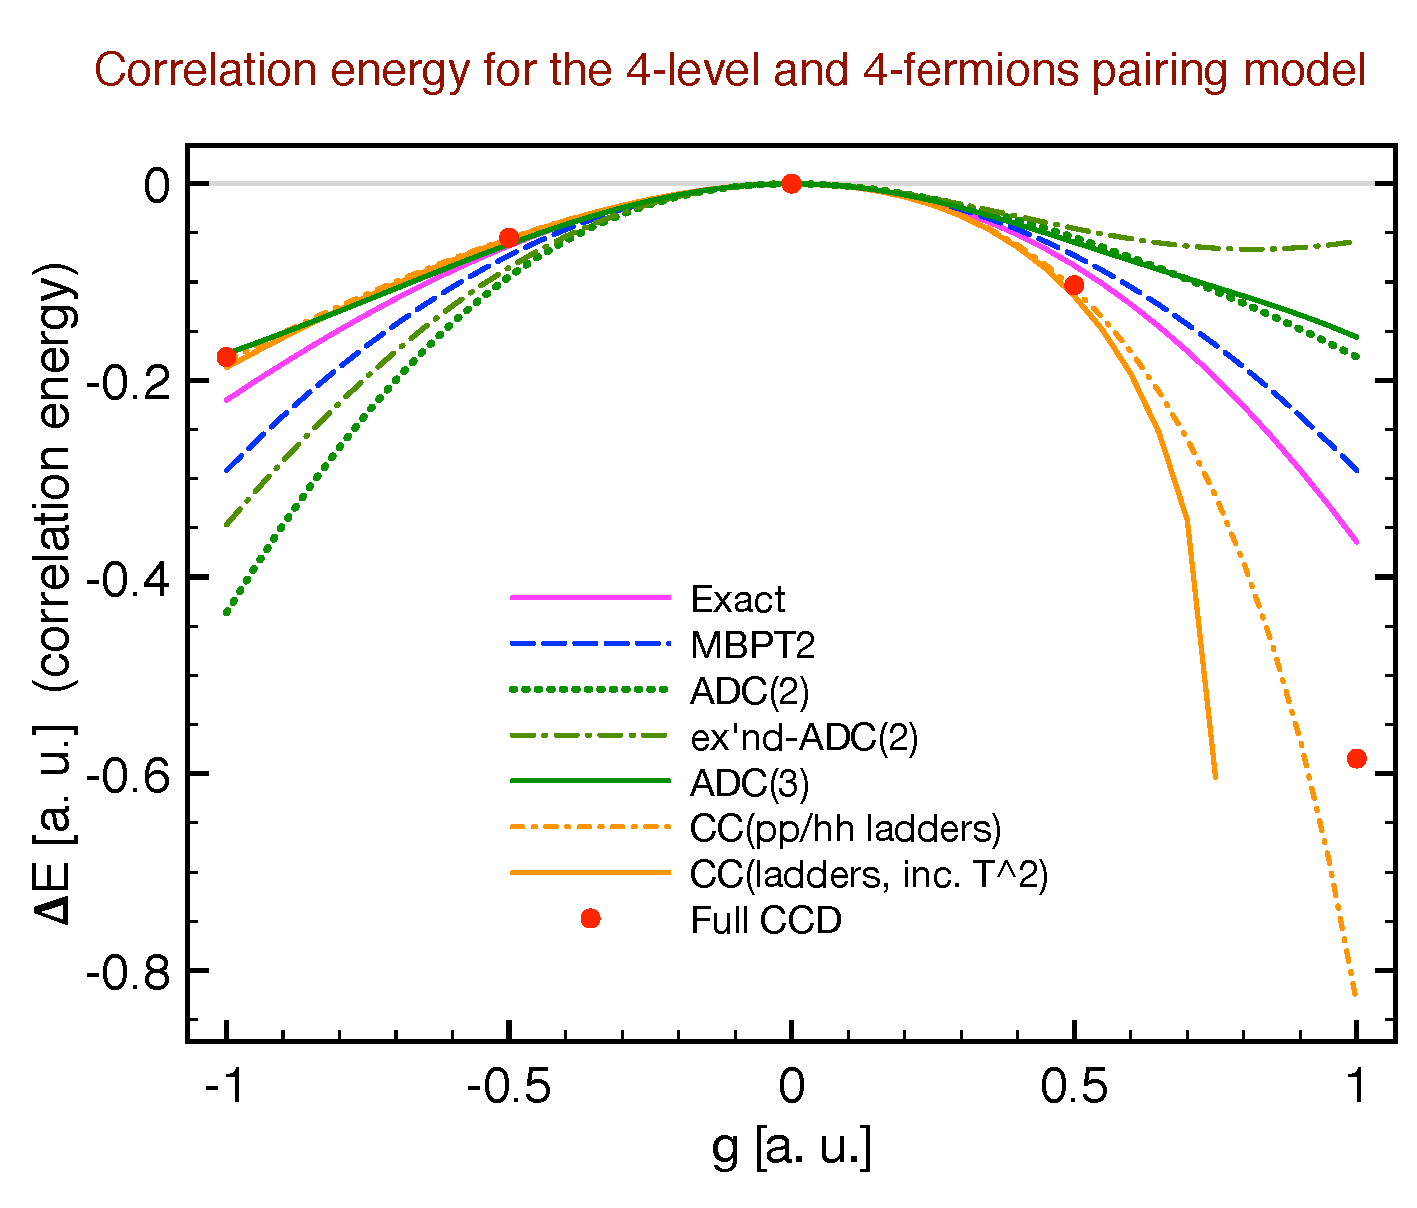
\includegraphics[width=0.8\textwidth]{Chapter11-figures/Pairing_model_CI_ADC_CC.pdf}
\caption{Correlation energy for the pairing Hamiltoninan of Eq.~\eqref{eq_pair_Ham} obtained for different
many body approximations. The purple line shows the exact results from full CI theory. Various CC approximation (as discussed in 
Chapter 8), the  ADC(2) and ADC(3) approximations are shown.}
\label{fig:pairng}
\end{center}
\end{figure}


\section{A computational project in infinite matter}
\label{sec:scgf_comp}


In this section we discuss how to approach  ADC(3) calculations of infinite matter. We will do this 
using the C++ programming language and will refer to the numerical code provided with in this chapter.

the most important deciosnin in order to set up a SCGF calcualtion is the choice of the model space. For
infinite matter, trasnlational inviariance imposes that the Dyson equation is diagonal in momentum  and 
therefore it becomes much easier to solve the problem in momentum space. However, there remain two possible
choices for how to encode the single particle degrees of freedom. 
The first one is to subdivide the infiite space in  boxes of finite lenth  and to impose periodic bounduarry conditions
(see also Chapter 8). In this way, the number of fermions included in each box is finite and determined by the particle
density of the system. The resulting model space is naturally expressed by a set of discretised single particle 
states and equations in the form of Eqs.~\eqref{eq:ADC3_MC}, \eqref{eq:ADC3_ND} and \eqref{eq:DysMtx}
can be solve directly as ti would be done for a finte system in a box.  Numerical results then need to be converged 
with respect to the trunction of the k-space inside each box.   We will follow this approach for the present 
computational project.
The other approach is to retain the full momentum space and write the SCGF equations already in the full 
thermodynamic limit. This approach is more suitable to solve the Dyson equation in at finite temperatures and
in a full SCGF fashion and will be discussed furtes in Sections~\ref{sec:scgf_finiteT} and~\ref{app:scgf_comp_finiteT}.


\vskip 0.5 cm
{\em Construction of the model space.}

\vskip 0.5 cm
{\em Construction of ISCs.}

\vskip 0.5 cm
{\em Two body interaction: Minnesota potential}

\vskip 0.5 cm
{\em Hartree-fock theory}

\vskip 0.5 cm
{\em Constructing the Dyson matrix}

\vskip 0.5 cm
{\em Numerical solutions at ASDC(20 and ADC(3) level}


\section{Self-consistenft GF at finite temperatures in the thermodynamic limit}
\label{sec:scgf_finiteT}

In the following we want to concentrate on the study of an infinite system at finite temperature; we will then set ourselves in the thermodynamic limit, i.e. number of particles $N$ and volume $V$ tending at infinity with density $\rho=N/V$ kept constant. The may-body SCGF approach at finite temperature is particularly suited for this kind of study because it is thermodynamically consistent, meaning that a quantity calculated from the microscopic point of view yields the same results as the thermodynamical macroscopic quantity [Baym62]. This consistency is strictly related to the fact that a fully dressed propagator, obtained via iterative solution of Dyson's equation, is used in the calculation of the partition function in the Luttinger-Ward formalism[Kohn-Luttinger59,Luttinger-Ward60], to obtain the thermodynamical properties of the system. Furthermore, it can be demonstrated that this method fulfils the Hugenholtz van-Hove theorem[vanHove58], and this once again relates to the fact that the conservation laws of particle number, momentum and energy are preserved in this kind of approximation [Baym61,62].

We will show how to calculate the self-consistent propagator in the ladder approximation, where particle-particle and hole-hole intermediate scattering states are resummed in the in-medium T-matrix, and then use the Koltun sumrule to obtain the total energy of the many-body system. Via the Luttinger-Ward formalism, the entropy can be calculated via the knowledge of the self-consistent propagator, and from the entropy all other thermodynamical quantities are accessible. We will first give a few hints on the theoretical formalism and then sketch the working equations necessary to perform the numerical calculation in the following section. The full self-consistent numerical calculation considering the complete off-shell properties of the system and considering fully microscopic potentials was performed independently by the Cracow group [Som�] and by the T�bingen/Barcelona group [Frick,Rios].

We start by defining the one-body Green's function as a statistical average in the grand-canonical ensemble:
\begin{equation}
\label{thermalG}
iG({\bf x}t, {\bf x'}t')= {\rm Tr}\{\hat{\rho}{\cal T}[\hat\psi({\bf x}t) \hat\psi^\dagger({\bf x'}t')]\}\,,
\end{equation}
where ${\cal T}$ describes the Wick time-ordered product of the quantum field operators of creation and destruction of a SP state, $\hat\psi^\dagger({\bf x'}t')$ and $\hat\psi({\bf x}t)$ respectively. The field operators are related to the operators of creation and destruction, i.e. $c^\dagger_k$ and $c_k$, via $\hat\psi^\dagger({\bf x'}t')=\sum_k\psi({\bf x}t)^\dagger c^\dagger_k$ and $\hat\psi({\bf x}t)=\sum_k\psi({\bf x}t)c_k$, where the coefficients are the single-particle wave functions and the sum is over the complete set of single-particle quantum numbers. For simplicity the variable ${\bf x}$ defines altogether the position, spin and isospin quantum numbers of a SP state, so an integration over ${\bf x}$ implies an integration over the position ${\bf x}$ and a summation over spin/isospin numbers. The statistical factor $\hat \rho$ is defined by:
\begin{equation}
\hat \rho=\frac{1}{Z}e^{-\beta(\hat H -\mu\hat N)}\,,
\end{equation}
where $\beta=1/T$, and $Z$ is the grand-partition function
\begin{equation}
Z={\rm Tr}\,e^{-\beta(\hat H -\mu\hat N)}\,,
\end{equation}
with $\hat H$ and $\hat N$ the hamiltonian and the particle number operators respectively. The trace in Eq.~(\ref{thermalG}) is to be taken over a full set of energy and particle number eigenstates of the system. The two possible time-ordering products in Eq.~(\ref{thermalG}) are given by:
\begin{equation}
\label{Tproduct}
{\cal T}[\hat\psi({\bf x}t) \hat\psi^\dagger({\bf x'}t')]=
 \Bigg\{
  \begin{tabular}{c}
  \,\,\,\,$\hat\psi({\bf x}t) \hat\psi^\dagger({\bf x'}t'), \quad t>t'$  \\
  $-\hat\psi^\dagger({\bf x'}t') \hat\psi({\bf x}t), \quad t'>t$
  \end{tabular}
\end{equation}
The first time-ordered product in Eq.~(\ref{Tproduct}) describes the creation of a particle state at time $t'$ with quantum numbers ${\bf x'}$, and the destruction of the propagated particle state at time $t$ with quantum numbers ${\bf x}$. Analogously, the second time-ordered product in Eq~(\ref{Tproduct}) describes the destruction of a particle state, or creation of a hole state, at time $t$ with quantum numbers ${\bf x}$, and the creation of the propagated hole state at time $t'$ with quantum numbers ${\bf x'}$. From Eq.~(\ref{Tproduct}) one can define the correlation functions: 
\begin{eqnarray}
\label{corr_creat}
iG^>({\bf x}t, {\bf x'}t')&=& {\rm Tr}\{\hat{\rho}[\hat\psi({\bf x}t) \hat\psi^\dagger({\bf x'}t')]\} \\
iG^<({\bf x}t, {\bf x'}t')&=& -{\rm Tr}\{\hat{\rho}[\hat\psi^\dagger({\bf x'}t')\hat\psi({\bf x}t)]\}\,.
\label{corr_destr}
\end{eqnarray}
Depending on the specific time ordering, the Green's function defined in Eq.~(\ref{thermalG}) corresponds to one correlation function or the other. It is also useful to define the retarded propagator. This is that part of the one-body Green's functions which is related only to the causal  propagation of events, i.e. forward in time:
\begin{equation}
\label{retar_prop}
G^R({\bf x}t, {\bf x'}t')=\theta(t-t')[G^>({\bf x}t, {\bf x'}t')-G^<({\bf x}t, {\bf x'}t')]\,.
\end{equation}

If we look at the quantum field operators of creation and destruction defined in the Heisenberg picture
\begin{equation}
\label{atemp}
\hat\psi({\bf x}t)=e^{i\hat Ht}\hat\psi^\dagger({\bf x}0)e^{-i\hat Ht}\,
\end{equation}
it is then possible to observe a resemblance between the thermal weight factor $e^{\beta\hat H}$ and the time evolution operator $e^{i\hat Ht}$ when considering the imaginary time domain $t=-i\beta$. If one includes the expression (\ref{atemp}) in the definition of the correlation functions Eqs.(\ref{corr_creat}) and (\ref{corr_destr}), it can then be checked that for a certain imaginary time domain there is absolute convergence of the two expressions, specifically in the intervals $-i\beta<t-t'<0$ for $G^>$ and $0<t-t'<i\beta$ for $G^<$. Furthermore, it can be shown that the two correlation functions are related to one another at one of their imaginary time boundaries, providing the important relation: 
\begin{equation}
\label{qprelation}
G^<({\bf x},t=0;{\bf x'}, t')=e^{\beta\mu}G^>({\bf x},t=-i\beta;{\bf x'},t')\,.
\end{equation}
Thanks to the translational invariance under space and time of an infinite system, the Green's function only depends on the differences ${\bf r}={\bf x'}-{\bf x}$ and $\tau=t-t'$. Exploiting the quasi-periodicity relation of the Green's function along the imaginary time axis given in Eq.~(\ref{qprelation}), one can write a discrete Fourier representation in the frequency domain:
\begin{equation}
G({\bf r},\tau)=\int \frac{{\rm d}^3p}{(2\pi)^3}e^{i{\bf p}{\bf r}}\frac{1}{-i\beta}\sum_\nu e^{-iz_\nu\tau}G({\bf p},z_\nu)\,,
\end{equation}
where $z_\nu=\frac{\pi\nu}{-i\beta}+\mu$ are the Matsubara frequencies. The Fourier coefficients are then given by the inverse transformation:
\begin{equation}
\label{Fouriercoeff}
G({\bf p},z_\nu)=\int {\rm d}^3r\int_0^{-i\beta}{\rm d}\tau\,e^{-i{\bf p}{\bf r}+iz_\nu\tau}G({\bf r},\tau)\,.
\end{equation}
These coefficients are evaluated for an infinite set of complex frequencies, corresponding to the imaginary time domain, however one would like to understand the properties of the physical propagator, i.e. in the real time and frequencies domain. To do so let's go back to the expressions of the correlation functions and write down their Fourier transform:
\begin{eqnarray}
\label{FTpart}
G^>({\bf p},\omega) &=& i\int{\rm d}^3r\int_{-\infty}^{+\infty}{\rm d}\tau\,e^{-i{\bf pr}+i\omega t}G^>({\bf r},\tau)\,,\\
\label{FThole}
G^<({\bf p},\omega) &=& -i\int{\rm d}^3r\int_{-\infty}^{+\infty}{\rm d}\tau\,e^{-i{\bf pr}+i\omega t}G^<({\bf r},\tau)\,.
\end{eqnarray}
These two quantities now define the spectral probability to attach or remove a particle with an energy $\omega$ from the momentum state {\bf p} of the many-body system (we now omit for simplicity the spin/isospin quantum numbers). The sum of these two functions defines a positive quantity which we call the spectral function:
\begin{equation}
\label{spec_fun}
A({\bf p},\omega)=G^>({\bf p},\omega)+G^<({\bf p},\omega)\,.
\end{equation}
An important feature of the spectral function is that it fulfils the sumrule
\begin{equation}
\int_{-\infty}^{+\infty}\frac{{\rm d}\omega}{2\pi}A({\bf p},\omega)=1\,,
\end{equation} 
this is also a reason why one can speak about probabilities when referring to the spectral function. 

Inserting Eqs.(\ref{FTpart}) and (\ref{FThole}) in Eq.~(\ref{qprelation}), we can write the Fourier transform of the periodicity condition
\begin{equation}
G^>({\bf p},\omega)=e^{\beta(\omega-\mu)}G^<({\bf p},\omega)\,,
\end{equation}
and considering the definition of the spectral function, we can write the correlation functions in momentum/frequency:
\begin{eqnarray}
\label{FTpart}
G^<({\bf p},\omega) &=& f(\omega)A({\bf p},\omega)\,,\\
\label{FThole}
G^<({\bf p},\omega) &=&[1-f(\omega)]A({\bf p},\omega)\,,
\end{eqnarray}
where $f(\omega)=\frac{1}{1+e^{\beta(\mu-\omega)}}$ is the Fermi-Dirac distribution function. These expression show that once the spectral function is known it is easy to access the correlation functions. It is then also possible to write a similar expression for the Fourier coefficients defined in Eq.(\ref{Fouriercoeff}):
 \begin{equation}
\label{FT_fullprop}
G({\bf p},z_\nu)=\int^{+\infty}_{-\infty} \frac{{\rm d}\omega'}{2\pi} \frac{A({\bf p},\omega')}{z_\nu-\omega'}\,.
\end{equation}
The previous expression is performed for an infinite set of frequencies in the imaginary time domain. However one would like to extend this to the entire complex plane, especially close to the real-time domain. It can be demonstrated that this analytical continuation is possible and one can safely replace $z_\nu=z$. [Baym61]. This property that relates the Green's function $G({\bf p},z)$ in the complex plane to the spectral function $A({\bf p},\omega)$ is called the spectral decomposition of the single-particle propagator. A similar Fourier transform can be written for the retarded propagator defined in Eq.~(\ref{retar_prop}):
 \begin{equation}
\label{FT_retarprop}
G^R({\bf p},\omega)=\int^{+\infty}_{-\infty} \frac{{\rm d}\omega'}{2\pi} \frac{A({\bf p},\omega')}{\omega_+-\omega'}\,,
\end{equation}
with $\omega_+=\omega+i\eta$. At this point, exploiting the Plemelj identity,
\begin{equation}
\frac{1}{\omega\pm i\eta}=\frac{\cal P}{\omega}\mp i\pi\delta(\omega)\,,
\end{equation}
one can separate the real and imaginary part of the retarded propagator, and it can be checked that the imaginary part of the retarded propagator coincides with the spectral function up to a factor:
\begin{equation}
\label{spec_img}
A({\bf p},\omega)=-2{\rm Im}G({\bf p},\omega_+)\,.
\end{equation}
By introducing the algebraic form of Dyson's equation:
\begin{equation}
G({\bf p},\omega_+)=\frac{1}{[G_0({\bf p},\omega_+)]^{-1}-\Sigma^\star({\bf p},\omega_+)}\,,
\label{G_algebraic}
\end{equation}
into Eq.~(\ref{spec_img})
one can express the spectral function as:
\begin{equation}
A({\bf p},\omega)=\frac{-2\mathrm{Im}\Sigma^\star({\bf p},\omega_+)}
{[\omega-\frac{p^2}{2m}-\mathrm{Re}\Sigma^\star({\bf p},\omega)]^2+[\rm{Im}\Sigma^\star({\bf p},\omega_+)]^2} \,.
\label{spectral_fun}
\end{equation}
The numerical self-consistent solution that one has to perform is the one given by Eq.~(\ref{spectral_fun}). This means that one performs an iterative calculation up to the point when the spectral function inserted in the calculation of the irreducible self-energy is equal to the one obtained by solving Eq.~(\ref{spectral_fun}).

Before going on, it is interesting to see that in the limit of zero temperature, the spectral decomposition of the one-body propagator given in Eq.~(\ref{FT_fullprop}) can be written as:
\begin{equation}
G({\bf p},\omega)=\int_{\varepsilon_\textrm F}^\infty\mathrm d\omega'\frac{S^p({\bf p},\omega')}{\omega-\omega'+i\eta}
+\int_{-\infty}^{\varepsilon_\textrm F}\mathrm d\omega'\frac{S^h({\bf p},\omega')}{\omega-\omega'-i\eta}\,,
\label{Lehm_infty}
\end{equation}
The $S^p({\bf p},\omega)$ and $S^h({\bf p},\omega)$ correspond to the particle and hole spectral functions respectively. Notice that we have now introduced one single Fermi energy $\varepsilon_\textrm F$ ($\varepsilon_\textrm F$ = $\varepsilon_\textrm F^+$ = $\varepsilon_\textrm F^-$) which, in an uncorrelated system, defines the last filled energy level and hence corresponds to the energy needed to remove a particle from the many-body ground state. In the case of an interacting system, not in the superfluid nor in the superconducting phase, $\varepsilon_\textrm F$ equals the chemical potential $\mu$, and corresponds to the minimum energy necessary to add or remove a particle to/from the many-body system. Consequently, the expression for the spectral function given in Eq.~(\ref{spectral_fun}) can be divided into two parts:
\begin{eqnarray}
S^p({\bf p},\omega)&=&-\frac{1}{\pi}\frac{\mathrm{Im}\Sigma^\star({\bf p},\omega)}
{(\omega-\frac{p^2}{2m}-\mathrm{Re}\Sigma^\star({\bf p},\omega))^2+(\rm{Im}\Sigma^\star({\bf p},\omega))^2} \quad \omega>\varepsilon_\textrm F\,,\qquad\,\,\,
\label{Sp_self}
\\ 
S^h({\bf p},\omega)&=&\frac{1}{\pi}\frac{\mathrm{Im}\Sigma^\star({\bf p},\omega)}
{(\omega-\frac{p^2}{2m}-\mathrm{Re}\Sigma^\star({\bf p},\omega))^2+(\rm{Im}\Sigma^\star({\bf p},\omega))^2} \quad\,\,\,\, \omega<\varepsilon_\textrm F\,.\quad
\label{Sh_self}
\end{eqnarray}

In the next subsection we will briefly sketch the steps that have to be taken to perform the numerical implementation of Eq.~(\ref{spectral_fun}) at finite temperature.

\subsection{Numerical implementation at finite temperature}
We show in Fig.~\ref{num_impl} a schematic representation of how the code works when considering both 2B and 3B forces. %Depending on the starting point of the iteration procedure, $\sim15$ iterations are needed to obtain converged results. These could be less for low densities and high temperatures, and if the starting point is a converged iteration for another density, temperature state of the system. The number of iterations for convergence increase for lower temperatures and high densities. 
The fundamental quantities that one has to calculate are the first-order two-body Green's function, the in-medium $T$-matrix and the irreducible self-energy, which are depicted in the the three blue boxes in Fig.~\ref{num_impl} with their respective Feynman diagrams. Following Feynman rules, diagrams are a direct way to write down the mathematical expressions that one has to solve numerically. For clarity, we will distinguish between the wording \emph{calculation} and \emph{iteration}: we will refer to \emph{calculation} as the set of several \emph{iterations} necessary to get to a converged results for the spectral function, so an \emph{iteration} is exactly what is depicted in Fig.~~\ref{num_impl}. For a more in depth explanation of the numerical details the reader can refer to [Frickthesis,Riosthesis].

 
\begin{figure}[t]
\begin{center}
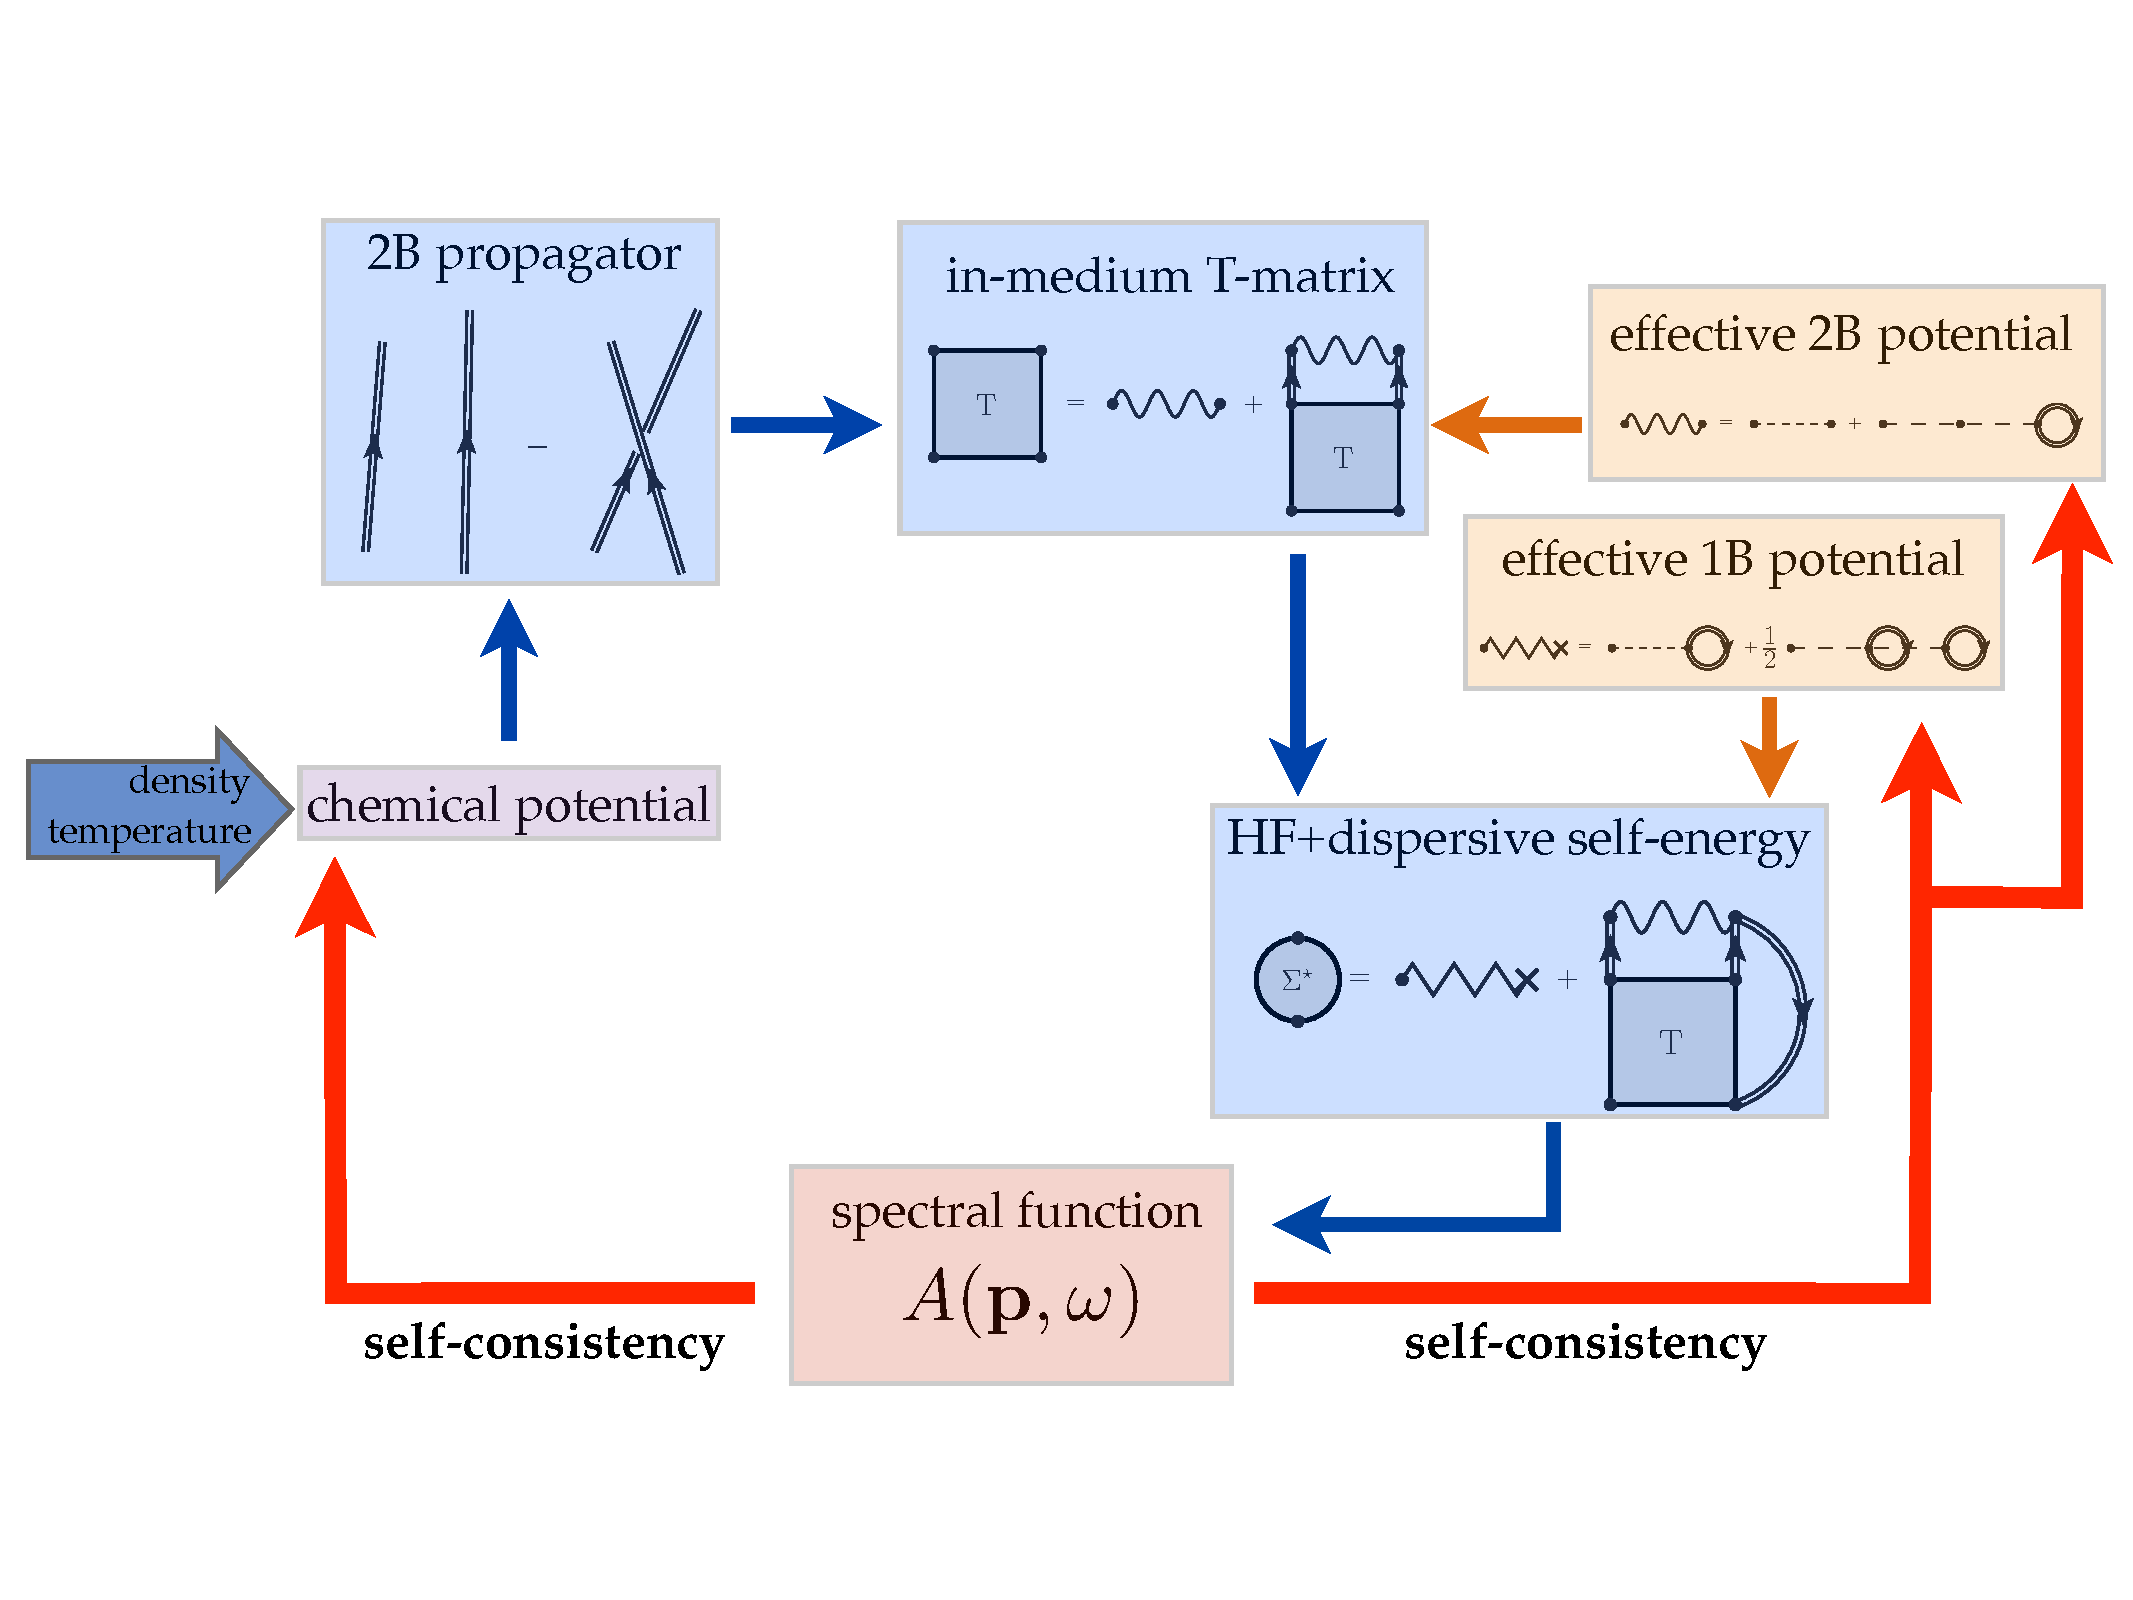
\includegraphics[width=1.0\textwidth]{Chapter11-figures/numerical_scgf_diagrams.pdf}
\caption{The structure of a ladder SCGF calculation including both 2BFs and 3BFs. Each quantity is also represented via a Feynman diagram.}
\label{num_impl}
\end{center}
\end{figure}


One starts the calculation from the thick external left arrow in Fig.~\ref{num_impl}, which corresponds to the input quantities: the density $\rho$ and temperature $T$ of the system. These, together with the imaginary, Im$\Sigma^*({\bf p},\omega)$, and real part, Re$\Sigma^*({\bf p},\omega)$, of the irreducible self-energy and the single-particle spectrum $\varepsilon({\bf p})$ obtained from a previous converged calculation are the ingredients to start with. 
\begin{itemize}
\item {\bf Mesh tips:}
The mesh of the single-particle momentum ${\bf p}$ for the self-energy is adjusted during the first iteration to be more dense around the Fermi momentum $p_{\rm F}$ corresponding to the specific density considered: $N_{\bf p}=70$ mesh points are enough, considering linear meshes at low momentum and around the Fermi momentum, and a logarithmic mesh for the tail all the way up to a value $\sim10p_{\rm F}$. The mesh in the single-particle energy $\omega$ has to be very dense because of the complicated features of the spectral function, especially at the quasi-particle peak. However storing a dense mesh at each iteration is demanding in terms of memory; for this reason one saves separately the imaginary and real part in a sparse mesh, $N_{\omega}=~6000$ linear mesh points from [-2000:15000] MeV, and then interpolates these quantities during the iterations to a denser meshes, $N_{\omega}=~30000$ linear mesh points, in order to have a good description of the spectral function in the energy domain. However, as it will be explained later on, the mesh in energy is adjusted in different ways during the iteration according to the specific quantities that one has to calculate (two-body propagator, T-matrix, etc.).
\end{itemize}

\noindent {\bf 1.} The density, temperature, spectral function and single-particle spectrum are the inputs to calculate the first quantity: the chemical potential. This is done by considering the relation:
\begin{equation}
\rho=\nu\int\frac{{\rm d}{\bf p}}{2\pi^3}\int_{-\infty}^{+\infty}\frac{{\rm d}{\omega}}{2\pi}A({\bf p},\omega)f(\omega,\mu)\,.
\label{chempot_micro}
\end{equation}
\begin{itemize}
\item {\bf Mesh tips:} One chooses a mesh of chemical potentials to insert in the Fermi-Dirac function $f(\omega,\mu)$ and solves the equation to find the one that matches the value of the external density. The mesh can be initially distributed around the value of the single-particle spectrum calculated at $p_{\rm F}$ (in the case of a zero temperature calculation it holds the relation $\varepsilon(p_{\rm F})=\mu$), and then adjusted testing if the limits include the value of the external density. However, it must be noted that the $\varepsilon({\bf p})$ comes from a different calculation, as also the chemical potential which enters the spectral function, so its has to be kept in mind that in the solution of Eq.~(\ref{chempot_micro}) one is considering two different chemical potentials, which will end up coinciding at the end of the convergence loop.
\end{itemize}

\noindent {\bf 2.} From the chemical potential one solves a self-consistent equation in the energy to find a new single-particle spectrum:
\begin{equation}
\varepsilon({\bf p})=\frac{p^2}{2m}+{\rm Re}\Sigma({\bf p},\varepsilon({\bf p}))\,,
\end{equation}
this will be used throughout the iteration. 
 
\noindent{\bf 3.} At this point the imaginary part of the first-order two-body Green's function can be calculated. The first order approximation of the two-body propagator corresponds to the independent propagation of two fully dressed particles. This includes two terms, a direct and an exchange one, (as depicted diagrammatically in Fig.~\ref{num_impl}). The imaginary part of this quantity reads:
\begin{equation}
\label{gII_imag}
{\rm Im}G^{II,f}_{pphh}(\Omega_+;{\bf p},{\bf p'}) = -\frac{1}{2}\int_{-\infty}^{+\infty}\frac{{\rm d}{\omega}}{2\pi}A({\bf p},\omega)A({\bf p'},\Omega-\omega)[1-f(\omega)-f(\Omega-\omega)]\,.
\end{equation}
where $\Omega_+$ is the sum of the energies of the two particles considered close to the real axis. This expression is derived from a sum over Matsubara frecuencies of a function with a double pole on the real-energy axis via use of the Cauchy theorem.
\begin{itemize}
\item {\bf Mesh tips:} The integrand of Eq.~(\ref{gII_imag}) will be particularly hard to resolve in the energy range where the two spectral functions are peaked. It can be demonstrated that performing a convenient variable change, one is safe with defining a mesh in energy accurately distributed around two specific regions, e.g. $\tilde\omega=0$ and $\tilde\omega=\tilde\Omega$ [for details see Ref.[Riosthesis]]. To obtain the spectral function in this specific mesh one interpolates the imaginary and real self-energies to this mesh and then solves Eq.~(\ref{spectral_fun}).
\end{itemize}

\noindent{\bf 4.} From the imaginary part it is then possible to obtain the real-part of the first-order two-body Green's function via a dispersion relation:
\begin{equation}
{\rm Re}G^{II,f}_{pphh}(\Omega_+;{\bf p},{\bf p'}) = -{\cal P}\int_{-\infty}^{+\infty}\frac{{\rm d}{\Omega'}}{\pi}\frac{{\rm Im}G^0_{II}(\Omega_+;{\bf p},{\bf p'})}{\Omega-\Omega'}]\,.
\end{equation}

\noindent{\bf 5.} An angle average is then necessary to calculate $G^{II,f}$. This average is necessary to circumvent the coupling of partial waves with different total angular momentum $J$ which appear in $G^{II,f}$. The average is performed over the angle formed by the center of mass momentum ${\bf P}$ and the relative momentum of the two nucleons ${\bf k}$. This strategy will facilitate the solution of the Lippmann-Schwinger equation to evaluate the effective interaction in the medium, known as the T-matrix. The average reads:
\begin{equation}
\overline{G^{II,f}_{pp,hh}}(\Omega;{\bf P},{\bf k})=\frac{1}{2}\int_{-1}^{+1}{\rm d\,cos}\theta G^0_{II}(\Omega;|{\bf P}/2+{\bf k}|,|{\bf P}/2-{\bf k}|)\,.
\end{equation}

\noindent{\bf 6.} The two-body angle-averaged propagator together with the nuclear potential are used to obtain the in-medium T-matrix. As explained previously, this is a ladder resummation of particle-particle and hole-hole diagrams, this differs with respect to the Brueckner G-matrix presented in Chapter 8 because it includes hole-hole diagrams and considers the full off-shell description of the spectral function. As seen from Fig.~\ref{num_impl}, the potential to be included is the sum of a bare two-body potential and an averaged three-body one. Details on the numerical solution for the average are given in the next section, while working equations for 3N chiral forces will be given in Appendix 1. The Lippmann-Schwinger type equation to be solved reads:
\begin{equation}
\label{t-matrix}
\langle{\bf k'}|{\rm T}(\Omega_+,{\bf P})|{\bf k}\rangle=\langle{\bf k'}|V^{\rm 2N}+\tilde V^{\rm 3N}|{\bf k}\rangle+\int {\rm d}{\bf k_1}\langle{\bf k'}|V^{\rm 2N}+\tilde V^{\rm 3N}|{\bf k_1}\rangle\overline{G^{II,f}_{pp,hh}}(\Omega;{\bf P},{\bf k_1})\langle{\bf k_1}|{\rm T}(\Omega_+;{\bf P})|{\bf k}\rangle\,.
\end{equation}
This is a one dimensional integral equation for each allowed combination of $J,\,S,\,T$, and at most two coupled values of $L$, due to the tensor component of the nuclear interaction. By means of a discretization procedure, the equation for the $T$-matrix is converted into a complex matrix equation which can be solved via standard numerical techniques [Rios]. A matrix inversion has to be performed to solve this equation. This can be quite demanding if the dimension of the matrix is large. 
\begin{itemize}
\item {\bf Mesh tips:} It is important to sample in a correct manner the number of integration mesh points without loosing physical information. This is achieved by sampling conveniently the region where $G^{II,f}$ is maximum in the relative momentum, so for $\Omega>0$ close to the pole $k'=\sqrt{m\Omega}$, and the high relative momentum region where, due to correlations, $G^{II,f}$ might not be negligible. Furthermore there is a node for $\Omega=2\mu$ present in the $T$-matrix so an accurate mesh for the bosonic energies around this value is needed for the forthcoming calculation of the self-energy.
\end{itemize}
At low temperatures, the appearance of bound states signals the onset of the pairing instability. This would directly appear as a pole in the matrix which has to be inverted to solve the Lippmann-Schwinger equation, for ${\bf P}=0$ and $\Omega=2\mu$. However, this should be seen only below a critical temperature which is around $T_c\sim4$ MeV. The calculations should not go below this border line in temperature. Especially in the case of symmetric nuclear matter, convergence at this temperature and for increasing density starts to be slow and difficult to achieve. This is due to the neutron-proton pairing in the coupled $^3S_1-^3D_1$ channel. In pure neutron matter, where this channel is not available, convergence is good all the way up to high densities, even for low temperatures. 

\noindent{\bf 7.} The remaining step in the SCGF method is the calculation of the self-energy from the T-matrix. The first quantity to be obtained is the imaginary part of the self-energy, Im$\Sigma^\star$:
\begin{equation}
{\rm Im}\Sigma_L({\bf p},\omega_+)=\int\frac{{\rm d}{\bf p'}}{2\pi^3}\int_{-\infty}^{+\infty}\frac{{\rm d}{\omega'}}{2\pi}\langle{\bf pp'}|{\rm Im}{\rm T}(\omega+\omega'_+,{\bf P})|{\bf pp'}\rangle A({\bf p'},\omega')[f(\omega')+b(\omega+\omega')]\,;
\end{equation}
We recall that this expression is also obtained from a summation over Matsubara frequencies of a function with two poles on the real energy axis. 
\begin{itemize}
\item {\bf Mesh tips:} A momenta and energy integrals have to be performed, taking special care for the pole in energy of the Bose function $b(\Omega)$. This pole is canceled by the node we had previously mentioned in the T-matrix, for this reason we had already defined a convenient mesh for $\Omega$ around the node. 
\end{itemize}
 
\noindent{\bf 8}. The real part of the self-energy is then obtained by means of a dispersion relation from the imaginary part: 
\begin{equation}
{\rm Re}\Sigma_L({\bf p},\omega_+)=\Sigma_{HF}({\bf p})-{\cal P}\int_{-\infty}^{+\infty}\frac{{\rm d}{\lambda}}{\pi}\frac{{\rm Im}\Sigma_L({\bf p},\lambda_+)}{\omega-\lambda}\,.
\end{equation}
The HF part of the SP self-energy is then calculated directly from the potential and the single particle momentum distribution $n({\bf p})$:
\begin{equation}
\label{HF_self}
\Sigma_{HF}({\bf p})=\int\frac{{\rm d}{\bf p'}}{2\pi^3}\Big[\langle{\bf pp'}|V^{\rm 2N}|{\bf pp'}\rangle +\frac{1}{2}\langle{\bf pp'}|\tilde V^{\rm 3NF}|{\bf pp'}\rangle\Big] n({\bf p})
\end{equation}
To evaluate this quantity, the calculation of the momentum distribution is needed. Detailed description on how to calculate this quantity and numerical details are given in Sec. 1.5.3. 

Finally, via Eq.~(\ref{spectral_fun}) the spectral function can be obtained and the procedure starts again until a consistent result is achieved. According to the mesh points in which the spectral function is needed, the interpolation is done on the imaginary and real part of the self-energy, and not directly on the spectral function. This is done in order to avoid incorrect samplings of the structure of the spectral functions which could induce numerical inaccuracies. We must point out that the energy mesh for the evaluation of the spectral function must be accurate enough to reproduce not only the quasi-particle peak region, but furthermore the low and high-energy tails which characterize the spectral function.   

\subsection{Calculations of neutron matter at finite temperatures.}
\label{app:scgf_comp_finiteT}

\subsection{Numerical calculation when including three-body forces.}
As shown in Fig.~\ref{num_impl}, the inclusion of an averaged 3N forces enters the calculation, as it can also be seen from Eqs.~(\ref{t-matrix}) and (\ref{HF_self}). This average is performed as:
\begin{equation}
%\nn &&
\langle {\bf p'_1 p'_2}|\tilde V^\mathrm{3NF}|{\bf p_1 p_2}\rangle_A =
\mathrm{Tr}_{\sigma_3}\mathrm{Tr}_{\tau_3}
\int \frac{{\mathrm d}{\bf p}_3}{(2\pi)^3}n({\bf p}_3)f({\bf p'_1},{\bf p'_2},{\bf p'_3})
%\\ && \quad\quad\quad\quad\quad
\langle {\bf 1' 2' 3'}|W
(1-P_{13}-P_{23})
|{\bf 1 2 3}\rangle_{A_{12}}f({\bf p_1},{\bf p_2},{\bf p_3}) \,;
\label{dd3bf_new}
\end{equation}
the ket is antisymmetrized only with respect to particles {\bf 1} and {\bf 2}, i.e. ${\rm A}_{12}=(1-{\rm P}_{12})/2$, which is not affected by the averaging procedure; with ${\rm P}_{12}=(1+\boldsymbol \sigma_1\cdot\boldsymbol \sigma_2)(1+\boldsymbol \tau_1\cdot\boldsymbol \tau_2)/4$ we define the permutation operator of momentum and spin/isospin quantum numbers of particles {\bf 1} and {\bf 2}. The momentum distribution that appears in Eq.~(\ref{dd3bf_new}) can be obtained directly from the spectral function, via the relation:
\begin{equation}
\label{mom_dist}
n({\bf p})=\int_{-\infty}^{+\infty}\frac{{\rm d}\omega}{2\pi}A({\bf p},\omega)f(\omega)
\end{equation}

Let us give some details on the numerical implementation for the calculation of the density-dependent force:
\begin{itemize}
\item We start with the definition of the mesh necessary to calculate the integral over the internal momenta ${\bf p}_3$. Considering that we deal with a dressed distribution function $n({\bf p}_3)$ which may have populated states at high momentum, we need to cover momenta up to a certain high value in which it is sure that the $n({\bf p}_3)$ has reached zero. We define three Gauss-Legendre meshes respectively from $0$ to $p_\textrm F/3$, from $p_\textrm F/3$ to $p_\textrm F+p_\textrm F/3$, from $p_\textrm F+p_\textrm F/3$ to $3p_\textrm F$. Meshes are chosen to cover accurately the behavior of the distribution function from momenta lower to those higher than $p_\textrm F$. Finally, high momenta after $p_\textrm F$ are represented through a tangential mesh. We have 50  points in the Gauss-Legendre meshes, and 500 in the tangential one. 
\item For the external relative momenta, i.e. $k$ and $k'$, and the relative angle between them, i.e. $z$=cos$\theta$, we define gaussian meshes. For relative momenta we have $N_k=100$, for values from 0 to 1100 MeV. At $k\sim1000$ MeV it is certain that the potential is zero. After the complete evaluation of the density-dependent force $\tilde V^\textrm {3NF}$, we perform a tangential map of these values up to relative momenta $k\sim10^6$ MeV. A high-momentum mapping of the potential is necessary for the correct integration of the Lippmann-Schwinger equation to obtain the $T$-matrix [Rio2007PhD]f.
\item We need to calculate the momentum distribution function coming form the previous iterative step, so via solution of Eq.~(\ref{mom_dist}). At each iterative step, the values of the imaginary and real part of the self-energy are stored, for different points in the energy and momentum space. The number of points in the energy mesh is $N_\omega\sim6000$ for energies ranging from $\omega=[-2200:10000]$ MeV. For the momentum mesh we have $N_k=70$, for SP momenta going from 0 to 3000 MeV. We then interpolate through a spline the values of the imaginary and real part of the self-energy to a fine energy mesh of $N_{\omega,\textrm{spline}}=30000$. These values are used to define the spectral function (see Eq.~(\ref{spectral_fun})) necessary to evaluate Eq.~(\ref{mom_dist}). This last step is performed via a trapezoidal integral in the energy range. We then perform a linear interpolation of the obtained values of $n({\bf p})$ to the mesh of ${\bf p}_3$ defined for the integration of the quantities in the density-dependent force. Extrapolated values are set to zero.
\end{itemize}

For the evaluation of the total energy via the modified GMK sum rule given in Eq.~(GMK), we need to evaluate the expectation value of the 3B operator. At the moment this term is obtained only a the HF level. To obtain the 3B expectation value, we then perform an integration of the kind:
\begin{equation}
\frac{\langle W\rangle_\textrm{HF}}{A}=\frac{\nu}{\rho}\int \frac{{\rm d}{\bf p}}{(2\pi)^3}n({\bf p}) \frac{\Sigma^\star_{\tilde V^\textrm{3NF}}({\bf p})}{3}\,.
\label{3B_exp}
\end{equation}
In the previous expression, the HF self-energy for the 3B part, i.e. $\Sigma^\star_{\tilde V^\textrm{3NF}}$ corresponds to the second term on the right-hand side of Eq.~(\ref{HF_self}). 


\section{Concluding remarks}


\begin{acknowledgement}
We tank A. Cipollone, T. Duguet, W. H. Dickhoff, M. Hjorth-Jensen, K. Hebeler, H. Muther, A. Polls, A. Rios, J. Schirmer, V. Som\`a and many others...   for several enlightening discussions. 
%If you want to include acknowledgments of assistance and the like at the end of an individual chapter please use the \verb|acknowledgement| environment -- it will automatically render Springer's preferred layout.
\end{acknowledgement}
%
\section*{Appendix 1: Chiral NNLO three-nucleon forces}
\addcontentsline{toc}{section}{Appendix 1: Chiral NNLO three-nucleon forces}
\label{app:scgf_3NF}

In this appendix we perform the average given in Eq.~(\ref{dd3bf_new}) for the specific case of leading order 3N forces in the chiral effective filed theory expansion. At NNLO we have a a two-pion (TPE), one-pion (OPE) and contact 3N terms, given respectively by the following expressions:

\begin{equation}
W_\mathrm{TPE} =\sum_{i\neq j\neq k}  \frac{g_A^2}{8F_\pi^4}
\frac{(\boldsymbol\sigma_i\cdot{\bf q}_i)(\boldsymbol\sigma_j\cdot{\bf q}_j)}{({\bf q}_i^2 + M_\pi^2)
({\bf q}_j^2 + M_\pi^2)}
F_{ijk}^{\alpha\beta}\tau_i^{\alpha}\tau_j^{\beta}\,,
\label{tpe}
\end{equation}
\begin{equation}
W_\mathrm{OPE} = -\sum_{i\neq j\neq k} \frac{c_D g_A}{8F_\pi^4\Lambda_\chi}
\frac{\boldsymbol\sigma_j\cdot{\bf q}_j}{{\bf q}_j^2 + M_\pi^2}(\boldsymbol\tau_i\cdot\boldsymbol\tau_j)
(\boldsymbol\sigma_i\cdot{\bf q}_j)\,;
\label{ope}
\end{equation}
\begin{equation}
W_\mathrm{cont} =  \sum_{j\neq k} \frac{c_E}{2F_\pi^4\Lambda_\chi}
\boldsymbol\tau_j \cdot \boldsymbol\tau_k \,.
\label{cont}
\end{equation}
In the TPE 3B contribution of Eq.~(\ref{tpe}), the quantity $F_{ijk}^{\alpha\beta}$ is
\begin{equation}
F_{ijk}^{\alpha\beta}=\delta^{\alpha\beta} [-4M_\pi^2c_1+2 c_3{\bf q}_i\cdot{\bf q}_j]
+\sum_\gamma c_4\epsilon^{\alpha\beta\gamma}\tau^\gamma_k\boldsymbol\sigma_k\cdot[{\bf q}_i\times{\bf q}_j]\,.
\label{tpe_tensor}
\end{equation}
The force is regularized with a function that in Jacobi momenta reads:
\begin{equation}
f({\bf p_1},{\bf p_2},{\bf p_3})=f(p,q)=\exp{\left[-\frac{(p^2+3q^2/4)}{\Lambda^2_\textrm{3NF}}\right]^n}\,,
\end{equation}
where ${\bf p}=({\bf p}_1-{\bf p}_2)/2$ and ${\bf q}=2/3({\bf p_3}-({\bf p}_1+{\bf p}_2)/2)$ are identified only in this expression as the Jacobi momenta. $\Lambda_\textrm{3NF}$ defines the cutoff value applied to the 3NF in order to obtain a 3B contribution which dies down similarly to the 2B part one. The regulator function is applied both on incoming $({\bf p},{\bf q})$ and outgoing $({\bf p'},{\bf q'})$ Jacobi momenta. In the numerical calculation, the approximation of ${\bf P}=0$ is used to facilitate the solution of equations. \\

{\bf Symmetric Nuclear Matter.} Let's start with the isospin-symmetric case of nuclear matter. Evaluating Eq.~(\ref{dd3bf_new}) for the TPE term of Eq.~(\ref{tpe}) leads to three contracted in-medium 2B interactions.\\ %These are represented in Figs.~\ref*{TPE-1}-\ref*{TPE-3}. 
{\bf TPE-1:} The first term is an isovector tensor term, this corresponds to a 1$\pi$ exchange contribution with an in-medium pion propagator:
\begin{equation}
\tilde V_\mathrm{TPE-1}^\mathrm{3NF}=\frac{g_A\,\rho_f}{2 F_\pi^4}
\frac{(\boldsymbol\sigma_1\cdot{\bf q})(\boldsymbol\sigma_2\cdot{\bf q})}{[q^2 + M_\pi^2]^2}
\boldsymbol\tau_1\cdot\boldsymbol\tau_2[2 c_1M_\pi^2+ c_3\,q^2]\,.
\label{tpe_dd_1}
\end{equation}
$\rho_f$ defines the integral of the correlated momentum distribution function weighed by the regulator function $f({\bf p_1},{\bf p_2},{\bf p_3})$
\begin{equation}
\frac{\rho_f}{\nu}=\int \frac{{\mathrm d}{\bf p}_3}{(2\pi)^3}n({\bf p}_3)f({\bf p_1},{\bf p_2},{\bf p_3})\,,
\label{rho_f}
\end{equation}
where $\nu$ is the degeneracy of the system, $\nu=4$ in the isospin symmetric case. If the regulator function included in Eq.~(\ref{rho_f}) were not dependent on the internal integrated momentum $p_3$, the integral would reduce to the value of the total density of the system, $\rho$, divided by the degeneracy and multiplied by an external regulator function.\\ %Consequently, the expression in Eq.~(\ref{rho_f}) would exactly equal the one presented in Ref.~{JWHol2010}, even though in our case we use a correlated momentum distribution function, while a step function up to the Fermi level is used in the latter.
{\bf TPE-2:}The second term is also a tensor contribution to the in-medium NN interaction. It adds up to the previous term. %and contributes to $V^v_{\sigma q}$ in Eq.~(\ref{on-shell_vnn}). 
This term includes vertex corrections to the 1$\pi$ exchange due to the presence of the nuclear medium:
\begin{eqnarray}
%&& 
\tilde V_\mathrm{TPE-2}^\mathrm{3NF}&=& \frac{g_A^2}{8\pi^2F_\pi^4}
\frac{\boldsymbol\sigma_1\cdot{\bf q}\boldsymbol\sigma_2\cdot{\bf q}}{q^2 + M_\pi^2} \boldsymbol\tau_1\cdot\boldsymbol\tau_2
\\ \nonumber && 
\times
\Big\{-4c_1M_\pi^2\left[\Gamma_1(k)+\Gamma_0(k)\right]
%\\\nonumber &&  \qquad\qquad
-(c_3+c_4)\left[q^2(\Gamma_0(k)+2\Gamma_1(k)+\Gamma_3(k))+4\Gamma_2(k)\right]
%\\ && \qquad\qquad
+4c_4{\cal I}(k)\Big\}\,.
\label{tpe_dd_2}
\end{eqnarray}
We have introduced the functions $\Gamma_0(k), \Gamma_1(k), \Gamma_2(k), \Gamma_3(k), {\cal I}(k)$, which are integrals over a single pion propagator:
\begin{equation}
\label{gamma0}
\frac{\Gamma_0(k)}{(2\pi)^2}=\int\frac{{\mathrm d}{\bf p}_3}{(2\pi)^3}n({\bf p}_3)
\frac{1}{[{\bf k}\pm{\bf p}_3]^2 + M_\pi^2}f({\bf p_1},{\bf p_2},{\bf p_3})\,;
\end{equation}
\begin{equation}
\label{gamma1}
\frac{\Gamma_1(k)}{(2\pi)^2}=\frac{1}{k^2}\int\frac{\d{\bf p}_3}{(2\pi)^3}n({\bf p}_3)
\frac{\pm{\bf k}\cdot{\bf p_3}}{[{\bf k}\pm{\bf p}_3]^2 + M_\pi^2}f({\bf p_1},{\bf p_2},{\bf p_3})\,;
\end{equation}
\begin{equation}
\label{gamma2}
\frac{\Gamma_2(k)}{(2\pi)^2}=\frac{1}{2k^2}\int\frac{\d{\bf p}_3}{(2\pi)^3}n({\bf p}_3)
\frac{p_3^2k^2-({\bf k}\cdot{\bf p_3})^2}{[{\bf k}\pm{\bf p}_3]^2 + M_\pi^2}f({\bf p_1},{\bf p_2},{\bf p_3})\,;
\end{equation}
\begin{equation}
\label{gamma3}
\frac{\Gamma_3(k)}{(2\pi)^2}=\frac{1}{2k^4}\int\frac{\d{\bf p}_3}{(2\pi)^3}n({\bf p}_3)
\frac{3({\bf k}\cdot{\bf p_3})^2-p_3^2k^2}{[{\bf k}\pm{\bf p}_3]^2 + M_\pi^2}f({\bf p_1},{\bf p_2},{\bf p_3})\,;
\end{equation}
\begin{equation}
\label{i_integral}
\frac{{\cal I}(k)}{(2\pi)^2}=\int \frac{{\mathrm d}{\bf p}_3}{(2\pi)^3}n({\bf p}_3)
\frac{[{\bf p}_3\pm{\bf k}]^2}{[{\bf p}_3\pm{\bf k}]^2 + M_\pi^2}f({\bf p_1},{\bf p_2},{\bf p_3})\,.
\end{equation}
%These integrals are formally equal to those presented in Ref.~{JWHol2010}, but differ in that a dressed propagator is used in our average, and the expressions are weighed with an internal regulator function.
{\bf TPE-3:} The last TPE contracted term includes in-medium effects for a 2$\pi$ exchange 2B term. %This expression contributes to all operatorial structures of Eq.~(\ref{on-shell_vnn}). Specifically it contributes to the scalar central term $V^s_c$,  to the isovector spin-spin $V^v_\sigma$ and tensor term $V^v_{\sigma q}$, to the spin-orbit in both isoscalar $V^s_{SL}$ and isovector form $V^v_{SL}$, and to the isovector quadratic spin-orbit term $V^v_{\sigma L}$:
\begin{eqnarray}
\nonumber &&
\tilde V_\mathrm{TPE-3}^\mathrm{3NF}=\frac{g_A^2}{16\pi^2F_\pi^4}\Big\{
-12c_1M_\pi^2\big[2\Gamma_0(k)-G_0(k,q)(2M_\pi^2+q^2)\big]
\\\nonumber &&   %\quad
-c_3\big[8k_F^3-12(2M_\pi^2+q^2)\Gamma_0(k)
-6q^2\Gamma_1(k)+3(2M_\pi^2+q^2)^2G_0(k,q)\big] 
\\\nonumber &&  %\qquad
+ 4c_4 \boldsymbol\tau_1\cdot\boldsymbol\tau_2(\boldsymbol\sigma_1\cdot\boldsymbol\sigma_2\, q^2-\boldsymbol\sigma_1\cdot{\bf q}\boldsymbol\sigma_2\cdot{\bf q})
G_2(k,q)
\\\nonumber &&  %\qquad
-(3c_3+c_4\boldsymbol\tau_1\cdot\boldsymbol\tau_2)\,i(\boldsymbol\sigma_1+\boldsymbol\sigma_2)\cdot({\bf q}\times{\bf k})
\\\nonumber &&  \qquad \times
\big[2\Gamma_0(k)+2\Gamma_1(k)-(2M_\pi^2+q^2)G_0(k,q)+2G_1(k,q)\big]
\\\nonumber &&  %\qquad 
-12c_1M_\pi^2\,  i(\boldsymbol\sigma_1+\boldsymbol\sigma_2)\cdot({\bf q}\times{\bf k})
\big[G_0(k,q)+2G_1(k,q)\big]
\\\nonumber &&  %\qquad
+4c_4\boldsymbol\tau_1\cdot\boldsymbol\tau_2\boldsymbol\sigma_1\cdot({\bf q}\times{\bf k})\boldsymbol\sigma_2\cdot({\bf q}\times{\bf k})
\\ && \qquad\times
\big[G_0(k,q)+4G_1(k,q)+4G_3(k,q)\big]\Big\}\,.
\label{tpe_dd_3}
\end{eqnarray}
Here we have introduced the function $G_0(k,q)$, which is an integral over the product of two different pion propagators:
\begin{equation}
\frac{G_{0,\star,\star\star}}{(2\pi)^2}(k,q)=
\int \frac{{\mathrm d}{\bf p}_3}{(2\pi)^3}n({\bf p}_3)
\frac{\{p_3^0,p_3^2,p_3^4\}}{\big[[{\bf k}+{\bf q}+{\bf p}_3]^2+M_\pi^2\big]\big[[{\bf p}_3+{\bf k}]^2+M_\pi^2\big]}f(k,k,p_3)\,.
\label{G_0} 
\end{equation}
The functions $G_{\star}(k,q), G_{\star\star}(k,q)$ have been introduced to define the rest of the functions, $G_1(k,q), G_2(k,q)$ and $G_3(k,q)$:
\begin{equation}
\label{G_1}
G_1(k,q)=\frac{\Gamma_0(k)-(M_\pi^2+k^2)G_0(k,q)-G_\star(k,q)}{4k^2-q^2}\,,
\end{equation}
\begin{equation}
\label{G_1star}
G_{1\star}(k,q)=\frac{3\Gamma_2(k)+k^2\Gamma_3(k)-(M_\pi^2+k^2)G_\star(k,q)-G_{\star\star}(k,q)}{4k^2-q^2}\,,
\end{equation}
\begin{equation}
\label{G_2}
G_2(k,q)=(M_\pi^2+k^2)G_1(k,q)+G_\star(k,q)+G_{1\star}(k,q)\,,
\end{equation}
\begin{equation}
\label{G_3}
G_3(k,q)=\frac{\Gamma_1(k)/2-2(M_\pi^2+k^2)G_1(k,q)-2G_{1\star}(k,q)-G_\star(k,q)}{4k^2-q^2}\,.
\end{equation}
Note that $G_{1\star}(k,q)$ is needed only to define $G_2(k,q),\,G_3(k,q)$.\\

Integrating Eq.~(\ref{dd3bf_new}) for the OPE 3NF term, given in Eq.~(\ref{ope}), leads to two contributions.\\
{\bf OPE-1:} The first one is a tensor contribution which defines a vertex correction to a 1$\pi$ exchange NN term. It is proportional to the quantity $\rho_f$, similar to what was obtained for the TPE 3NF contracted term $\tilde V_\mathrm{TPE-1}^\mathrm{3NF}$ (see Eq.~\ref{tpe_dd_1}):
\begin{equation}
\tilde V_\mathrm{OPE-1}^\mathrm{3NF}=-\frac{c_D\,g_A\,\rho_f}{8\,F_\pi^4\,\Lambda_\chi}
\frac{(\boldsymbol\sigma_1\cdot{\bf q})(\boldsymbol\sigma_2\cdot{\bf q})}{q^2 + M_\pi^2}
(\boldsymbol\tau_1\cdot\boldsymbol\tau_2)\,.
\label{ope_dd_1}
\end{equation}
As for the $\tilde V_\mathrm{TPE-1}^\mathrm{3NF}$ term, $\tilde V_\mathrm{OPE-1}^\mathrm{3NF}$ it's an isovector tensor term.\\% $V^v_{\sigma q}$ of Eq.~(\ref{on-shell_vnn}).
{\bf OPE-2:} The second term derived from the 3NF OPE defines a vertex correction to the short-range contact NN interaction.  This in-medium interaction contribution is formed of terms of various kinds: a central scalar, a  spin-spin, a tensor and quadratic spin-orbit terms, all contributions in the isovector form. It reads:
\begin{eqnarray}
\nonumber &&
\tilde V_\mathrm{OPE-2}^\mathrm{3NF}=\frac{c_Dg_A}{16\pi^2F_\pi^4\Lambda_\chi}\Big\{
\big(\Gamma_0(k)+2\Gamma_1(k)+\Gamma_3(k)\big)
%\\\nonumber &&
\left[\boldsymbol\sigma_1\cdot\boldsymbol\sigma_2\Big(2k^2-\frac{q^2}{2}\Big)\right.
\\\nonumber && \left.\qquad
+(\boldsymbol\sigma_1\cdot{\bf q}\,\boldsymbol\sigma_2\cdot{\bf q})\Big(1-\frac{2k^2}{q^2}\Big)-\frac{2}{q^2}\boldsymbol\sigma_1\cdot({\bf q}\times{\bf k})
\boldsymbol\sigma_2\cdot({\bf q}\times{\bf k})\frac{1}{q^2}\right]
\\ && \qquad
+2\Gamma_2(k)(\boldsymbol\sigma_1\cdot\boldsymbol\sigma_2)\Big](\boldsymbol\tau_1\cdot\boldsymbol\tau_2)
+6{\cal I}(k)\Big\}\,.
\label{ope_dd_2}
\end{eqnarray}

{\bf Contact:} The last density-dependent term arises from a contraction of the contact 3NF term given in Eq.~(\ref{cont}). This yields a scalar central contribution to the in-medium NN interaction proportional to $\rho_f$. Hence, being momentum independent it will contribute only to $S$ partial waves. Its formal expression is:
\begin{equation}
\tilde V_\mathrm{cont}^\mathrm{3NF}=-\frac{3 c_E\rho_f}{2 F_\pi^4\Lambda_\chi}\,.
\label{cont_dd}
\end{equation}

%We would like to underline once more that the obtained in-medium NN interaction terms, Eqs.~(\ref{tpe_dd_1}), (\ref{tpe_dd_2}), (\ref{tpe_dd_3}), (\ref{ope_dd_1}), (\ref{ope_dd_2}) and (\ref{cont_dd}) are formally the same to those obtained by the authors in Ref.~{JWHol2010}. The difference lies in the integrals over a single and a product of pion propagators and in the function $\rho_f$. These integrals differ not only in that our averaging procedure is performed using the correlated momentum distribution function $n({\bf p}_3)$, but furthermore in the weighing of the integrand with the full regulator function $f(k,k',p_3)$ presented in Eq.~(\ref{reg_fun}). In the next section we will test the discrepancies obtained on the effective 2B potential given by different averaging procedures.


%%%%%%%%%%%% neutron matter %%%%%%%%%%%%%%%%%%%%%%
{\bf Pure Neutron Matter.} In the case of pure neutron matter, the evaluation of Eq.~(\ref{dd3bf_new}) is simplified. In fact,
the trace over isospin is trivial, neutron matter can only be in total isospin $T=1$, i.e. $\boldsymbol\tau_1\cdot\boldsymbol\tau_2=1$. Consequently the exchange operator reduces only to the momentum and spin part, i.e. in spin space it reads:
\begin{equation}
P_{12}=\frac{1+\boldsymbol\sigma_1\cdot\boldsymbol\sigma_2}{2}\,.
\label{perm_op_2}
\end{equation}
It can then be proved that in-medium terms proportional to $c_4, c_D, c_E$ go to zero [Tolos2008, Heb2010Jul, JWHol2010]. 

In fact, for the term proportional to $c_E$, the contact contribution in Eq.~(\ref{cont}), the permutation of spin indices leads to equal direct and exchange terms which directly cancel one another. Physically this is a consequence of the Pauli principle which neutrons, being fermions, must respect. In other words, $W_\textrm{cont}$ vanishes between antisymmetrized three-nucleon states.

For the OPE term proportional to $c_D$, Eq.~(\ref{ope}), it can be demonstrated that the spin-momentum structure of this contribution leads to a vanishing quantity when the trace over spin is applied (for further details see [Carbonethesis]). The physical reason lies in the fact that both spin and relative momentum state of the two-neutron system interacting via the contact term in Eq.~(\ref{ope}) is symmetric, which cannot be the case for an overall wave function for a two-fermion state. 

The other vanishing term, the $c_4$ part of the TPE contribution in Eq.~(\ref{tpe}), contains an operatorial structure of the kind $(\boldsymbol\tau_1\times\boldsymbol\tau_2)\cdot\boldsymbol\tau_3$, and further permutations of particles 1,3 and 2,3. This structure is zero in a three neutron system. 

Therefore the only density-dependent contributions, which are non-zero in neutron matter, are those proportional to LECs $c_1$ and $c_3$ in Eqs.~(\ref{tpe})-(\ref{tpe_tensor}). The density-dependent interacting terms obtained in neutron matter will only differ with respect to the symmetric case ones by different pre-factors. This is due to the fact that the only part which changes from the symmetric to the pure neutron matter case is the trace over isospin indices. 

In order to obtain the correct degeneracy for neutron matter, i.e.  $\nu=2$, we need to replace $\rho_f \rightarrow 2\rho_f$ in the $\tilde V_\mathrm{TPE-1}^\mathrm{3NF}$ contribution of Eq.~(\ref{tpe_dd_1}), (see also Eq.~(\ref{rho_f})). The isovector tensor terms $\tilde V_\mathrm{TPE-1}^\mathrm{3NF}$ and  $\tilde V_\mathrm{TPE-2}^\mathrm{3NF}$, given in Eqs.~(\ref{tpe_dd_1})-(\ref{tpe_dd_2}) must then change prefactor according to:
\begin{equation}
\tilde V_\mathrm{TPE-1}^\mathrm{3NF}: \boldsymbol\tau_1\cdot\boldsymbol\tau_2 \rightarrow \frac{1}{2}\boldsymbol\tau_1\cdot\boldsymbol\tau_2\,, 
\label{pnm_tpe_1}
\end{equation}
\begin{equation}
\tilde V_\mathrm{TPE-2}^\mathrm{3NF}: \boldsymbol\tau_1\cdot\boldsymbol\tau_2 \rightarrow 
\frac{1}{4}(\boldsymbol\tau_1\cdot\boldsymbol\tau_2-2)\,.
\label{pnm_tpe_2}
\end{equation}
The isoscalar part of the density-dependent potential appearing in $\tilde V_\mathrm{TPE-3}^\mathrm{3NF}$, which contributes to both a central and spin-orbit terms, must change prefactor according to:
\begin{equation}
\tilde V_\mathrm{TPE-3}^\mathrm{3NF}: 1 \rightarrow \frac{1}{3}\,.
\label{pnm_tpe_3}
\end{equation}


\section*{Appendix 2: Feynman rules for the one-body propagator and self-energy}
\addcontentsline{toc}{section}{Appendix 2: Feynman rules for the one-body propagator and self-energy}
\label{app:Feyn_rules}





\begin{thebibliography}{99.}%
% Contribution 
\bibitem{science-contrib} Broy, M.: Software engineering --- from auxiliary to key technologies. In: Broy, M., Dener, E. (eds.) Software Pioneers, pp. 10-13. Springer, Heidelberg (2002)
%
% Online Document
\bibitem{science-online} Dod, J.: Effective substances. In: The Dictionary of Substances and Their Effects. Royal Society of Chemistry (1999) Available via DIALOG. \\
\url{http://www.rsc.org/dose/title of subordinate document. Cited 15 Jan 1999}
%
% Monograph
\bibitem{science-mono} Geddes, K.O., Czapor, S.R., Labahn, G.: Algorithms for Computer Algebra. Kluwer, Boston (1992) 
%
% Journal article
\bibitem{science-journal} Hamburger, C.: Quasimonotonicity, regularity and duality for nonlinear systems of partial differential equations. Ann. Mat. Pura. Appl. \textbf{169}, 321--354 (1995)
%
% Journal article by DOI
\bibitem{science-DOI} Slifka, M.K., Whitton, J.L.: Clinical implications of dysregulated cytokine production. J. Mol. Med. (2000) doi: 10.1007/s001090000086 

\end{thebibliography}



